\section{Method}
\label{sec:method}

\subsection{Task, data and protocol}
\label{sec:method-protocol}

We evaluate on six categories of VisA (candle, capsules, cashew, chewinggum, fryum,
pipe\_fryum) in the few-shot setting, with 1, 2, 4 and 8 normal reference images per category
and three sampling seeds (0/1/2). For every category the first 20 training images are held
out as a \emph{calibration set} and never used as references; the remaining normal images
form the pool from which the $k$-th shot of the $s$-th seed is drawn
($\text{pool}[s \cdot \text{shot} : (s{+}1) \cdot \text{shot}]$), so every method sees
exactly the same references for a given (shot, seed). The same 960 test images are scored by
every system.

Two metrics are reported. Image-level AUROC uses the mean of the top 1\% of the pixel
distance map as the anomaly score, as in AnomalyDINO~\cite{damm2025anomalydino}. Pixel-level
AUROC is computed on maps resampled to $448\times448$ for all methods, because pooling the
native-resolution pixels of all images does not fit in the shared GPU memory; the same
resampling is applied everywhere, so comparisons stay well defined. Mean\,$\pm$\,std is always
taken over seeds: the six-category mean is formed per seed first, and the standard deviation
is taken over the three per-seed means. The decision threshold, used only for the
qualitative error analysis and the OK/NG operating points, is the 95th percentile of the
scores of the 20 calibration images -- it never sees a test label.
Figure~\ref{fig:pipeline} summarises the full pipeline.

\begin{figure*}[t]
  \centering
  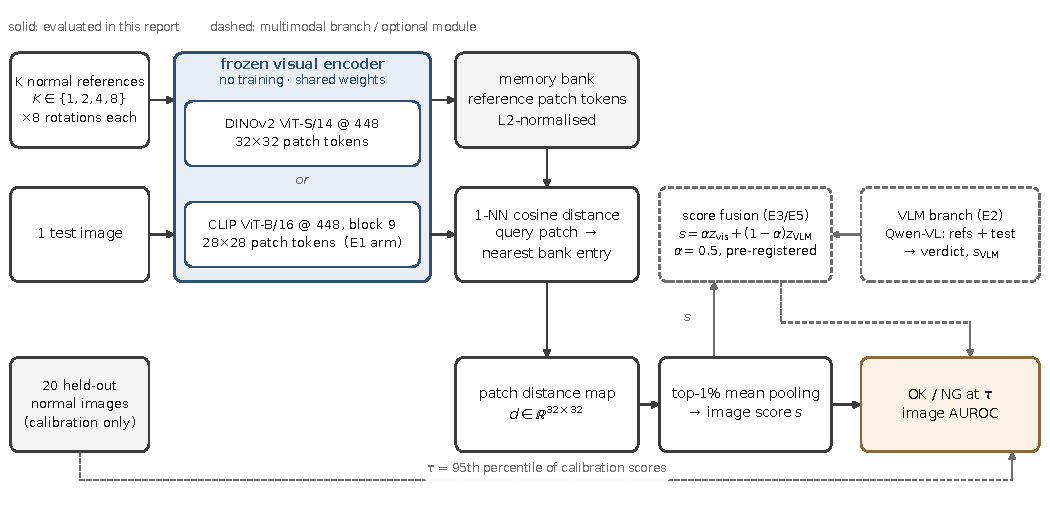
\includegraphics[width=\textwidth]{figures/pipeline.pdf}
  \caption{Overview of the pipeline under the frozen protocol. The support path builds an
  L2-normalised memory bank from $K$ normal references and their 8 rotations; the query path
  pushes the test image through the \emph{same} frozen encoder, scores every patch by 1-NN
  cosine distance against the bank, and pools the top 1\% of the distance map into the image
  score. The two encoders are interchangeable arms (E1) that share everything else. The
  dashed modules are optional: score-level fusion with the multimodal branch (E2--E5), and
  the decision threshold, which is derived from 20 held-out normal calibration images only.}
  \label{fig:pipeline}
\end{figure*}

\subsection{Part 1 -- template-difference baseline}
\label{sec:method-part1}

The baseline treats the reference set as a template. Images are resized so that the shorter
edge is 448 and centre-cropped, because a pixel-wise comparison needs a common frame; ECC
registration maps every image onto the first reference; the difference between a test image
and a reference is $0.5\,|\Delta I| + 0.5\,(1 - \mathrm{SSIM})$; the closest template (lowest
mean difference) becomes the anomaly map, which is Gaussian-smoothed and aggregated with the
same top-1\% mean as AnomalyDINO so that image AUROC stays comparable. Scores are never
rescaled per image. The baseline needs no training and no pretrained weights, and it fixes
the lower bound of the comparison: a pretrained-feature method that does not beat it is not
earning its complexity.

\subsection{Part 2 -- verified AnomalyDINO reproduction}
\label{sec:method-part2}

AnomalyDINO extracts dense patch features from DINOv2 ViT-S/14 at 448 ($32\times32$ patch
grid), builds a memory bank from the reference patches (each reference contributes eight
rotations, which makes the bank rotation-tolerant), and scores a test patch by its L2
distance to the nearest bank entry; the pixel map is the upsampled distance field, smoothed
with a Gaussian. We first reproduced this pipeline with the official code, then
re-implemented the scoring in a cached runner so that Part~3 variants can be compared without
re-extracting features.

The re-implementation is verified rather than assumed: a parity probe compares the two
pipelines cell by cell, and after the fixes described below all 72 cells (6 categories
$\times$ 4 shots $\times$ 3 seeds) agree with the official run to the last printed digit. Two
defects were found and fixed on the way, and both matter for Part~3:
\begin{enumerate}
  \item \textbf{Cache-key collision.} VisA reuses file names across splits (capsules shares
        eight basenames between \texttt{test/good} and \texttt{test/bad}, and ${\sim}90$
        between \texttt{train/good} and \texttt{test/bad}). A basename-keyed feature cache
        therefore served a defective image the features of a normal image with the same name,
        which cost up to 5 image-AUROC points on capsules. Cache keys are now namespaced by
        the parent directory.
  \item \textbf{Lossy cache dtype.} Storing cached features as float16 perturbed query
        features by up to ${\sim}8\times10^{-3}$, enough to change the top-1\% nearest
        neighbours of borderline images; the cache is now float32.
\end{enumerate}

\subsection{E1 -- replacing the backbone with CLIP}
\label{sec:method-e1}

The question E1 asks is narrow: with the scoring rule, the reference sampling, the
calibration and the resolution all held fixed, what changes when the dense features come from
a language-aligned image encoder (CLIP ViT-B/16) instead of a self-supervised one (DINOv2
ViT-S/14)? DINOv2 features are trained to be locally discriminative, which is what a
nearest-neighbour patch matcher wants; CLIP features are trained to place a whole image next
to a text description, and are known to be strongly anisotropic at the patch level. Whether
that costs accuracy in few-shot anomaly detection is an empirical question.

\paragraph{Extracting patch tokens from CLIP.}
\texttt{clip.encode\_image} returns only the pooled global feature, so the patch tokens are
taken from the vision tower directly: the input is patch-embedded, passed through the
transformer blocks, and for block $l$ we take the residual-stream output, drop the class
token, apply \texttt{ln\_post} and the projection matrix \texttt{proj} (so the vectors live
in the same space as the global embedding), and keep the remaining $g_h \times g_w$ tokens in
raster order. Three properties were verified explicitly, because a silent mistake in any of
them produces plausible-looking but wrong AUROC:
\begin{itemize}
  \item \textbf{Grid order.} A synthetic probe replaces one patch of the input with a white
        square; the argmax of the extracted tokens must be $\mathrm{row}\cdot14+\mathrm{col}$.
        It is ($5{\cdot}14{+}8 = 78$), confirming raster order.
  \item \textbf{Positional embedding at 448.} CLIP is trained at 224 with a $14{\times}14$
        position grid; a 448 input produces a $28{\times}28$ grid, so the learned position
        table is interpolated bicubically to the actual (rectangular) grid shape. An occlusion
        probe checks that the score map responds at the occluded location: the argmax lands
        within 3 patches of the true occlusion centre.
  \item \textbf{Forward equivalence.} For the native 224 input, our manual forward and the
        official \texttt{encode\_image} agree bit-for-bit on the class token, so the token
        extraction path introduces no off-by-one block or missing normalisation.
\end{itemize}
The resulting wrapper mirrors the DINOv2 interface
(\texttt{prepare\_image} $\rightarrow$ \texttt{extract\_layers}), which lets the same cached
scoring pipeline evaluate both backbones; no scoring code is duplicated.

\paragraph{Choices frozen before the grid.}
A pilot (candle and capsules, 1-shot, seed 0) fixed four settings; none were tuned on the
test split afterwards.
\begin{itemize}
  \item \textbf{Resolution 448, not 224.} The interpolated position table is stable at 448,
        so we keep the same resolution as Part~2 instead of falling back to CLIP's native
        224; the control is DINOv2 at 448.
  \item \textbf{Layer 9 of 12.} Patch features were swept over blocks 6, 9 and 12. The last
        block is the most anisotropic in CLIP (mean pairwise cosine similarity of patch
        features inside one image 0.57--0.67, against 0.36 for DINOv2 L12) and its dense
        matching suffers for it: at 1-shot on the pilot, block 12 scored 69.4 image AUROC on
        candle against 89.9 for block 9 under the same framing. Block 9 has the lowest
        anisotropy of the three and the best pixel AUROC under the frozen framing; blocks 6
        and 12 are reported as a sensitivity check, not as candidates.
  \item \textbf{No foreground mask, for both backbones.} AnomalyDINO's agnostic
        preprocessing estimates a foreground mask by PCA on DINOv2 features; the threshold is
        tied to that feature geometry and has no counterpart for CLIP. Rather than give one
        backbone a preprocessing advantage, E1 disables the mask for both, so the only
        difference between the two lines is the encoder.
  \item \textbf{\texttt{short\_edge} framing.} The official CLIP preprocessing centre-crops
        to a square, which cuts objects out of frame on categories whose objects are
        off-centre (capsules pixel AUROC dropped to 75.5 under the crop). \texttt{short\_edge}
        keeps the full frame and lets the patch grid be rectangular, matching the DINOv2
        wrapper; the same framing is used for both backbones.
\end{itemize}

\subsection{Fusion protocol and the multimodal branch}
\label{sec:method-fusion}

Fusion is pre-registered before any outcome is seen: each branch's score is standardised per
category with the median and MAD of its scores on the 20 held-out normal calibration images
(falling back to the standard deviation, then to a constant, when the MAD degenerates), and
the fused score is $\alpha z_1 + (1-\alpha) z_2$ with the main result at $\alpha = 0.5$; the
five-point $\alpha$ sweep is reported as a sensitivity analysis, never as a tuned optimum, and
no test label participates in any choice~\cite{guo2017calibration}. The machinery is checked
with a consistency requirement: $\alpha{=}1$ and $\alpha{=}0$ must reproduce the single
branches exactly. \bsec{E2: Qwen-VL branch description, prompts, decoding and per-image
scores} completes the taxonomy's fourth cell and feeds E3--E5.
